\chapter{Results}
\label{sec:intro_res}

To rigorously evaluate the performance of the metaheuristic, two distinct percentage gaps are computed:

\begin{itemize}
    \item \textbf{Gap vs Best:} Measures the deviation of the metaheuristic solution from the best feasible solution (Upper Bound) found by the exact algorithm.
    \begin{equation}
        \text{Gap}_{\text{Best}} (\%) = \frac{\text{Obj}_{\text{Meta}} - \text{Obj}_{\text{MIP}}}{\text{Obj}_{\text{MIP}}} \times 100
    \end{equation}
    
    \item \textbf{Gap vs LB (Worst-case Optimality Gap):} Measures the maximum possible deviation from the theoretical optimum, using the Lower Bound provided by the MIP solver. This metric is particularly useful for instances where the exact algorithm reaches the time limit without proving optimality.
    \begin{equation}
        \text{Gap}_{\text{LB}} (\%) = \frac{\text{Obj}_{\text{Meta}} - \text{LB}_{\text{MIP}}}{\text{LB}_{\text{MIP}}} \times 100
    \end{equation}
\end{itemize}

For instances solved to exact optimality within the time limit, the Best Objective and the Lower Bound coincide, rendering the two gap values identical.

All the results are shown in the \textbf{Table \ref{tab:results_comparison_lb}}.

\section[Table \ref{tab:results_comparison_lb} Analysis]{Table \ref{tab:results_comparison_lb} Analysis}

\subsection{Analysis of the obj. values}

\textbf{Histogram \ref{fig:obj_histogram_2}} and \textbf{Histogram \ref{fig:obj_histogram_1}} show the results in a histogram where  the number of the instance and its number of the jobs and of the machines is given. Here we can observe how the objective value of the MIP implementation at the beginning is equal to the metaheuristic value and the lower bound. These are the cases where the 300 seconds timer doesn't run out. As the number of jobs and machines increases, the MIP solver starts to reach the timer more frequently. So the solutions are found more rarely and, if found, are very far from the LB and the metaheuristic ones.

\begin{figure}
    \centering
    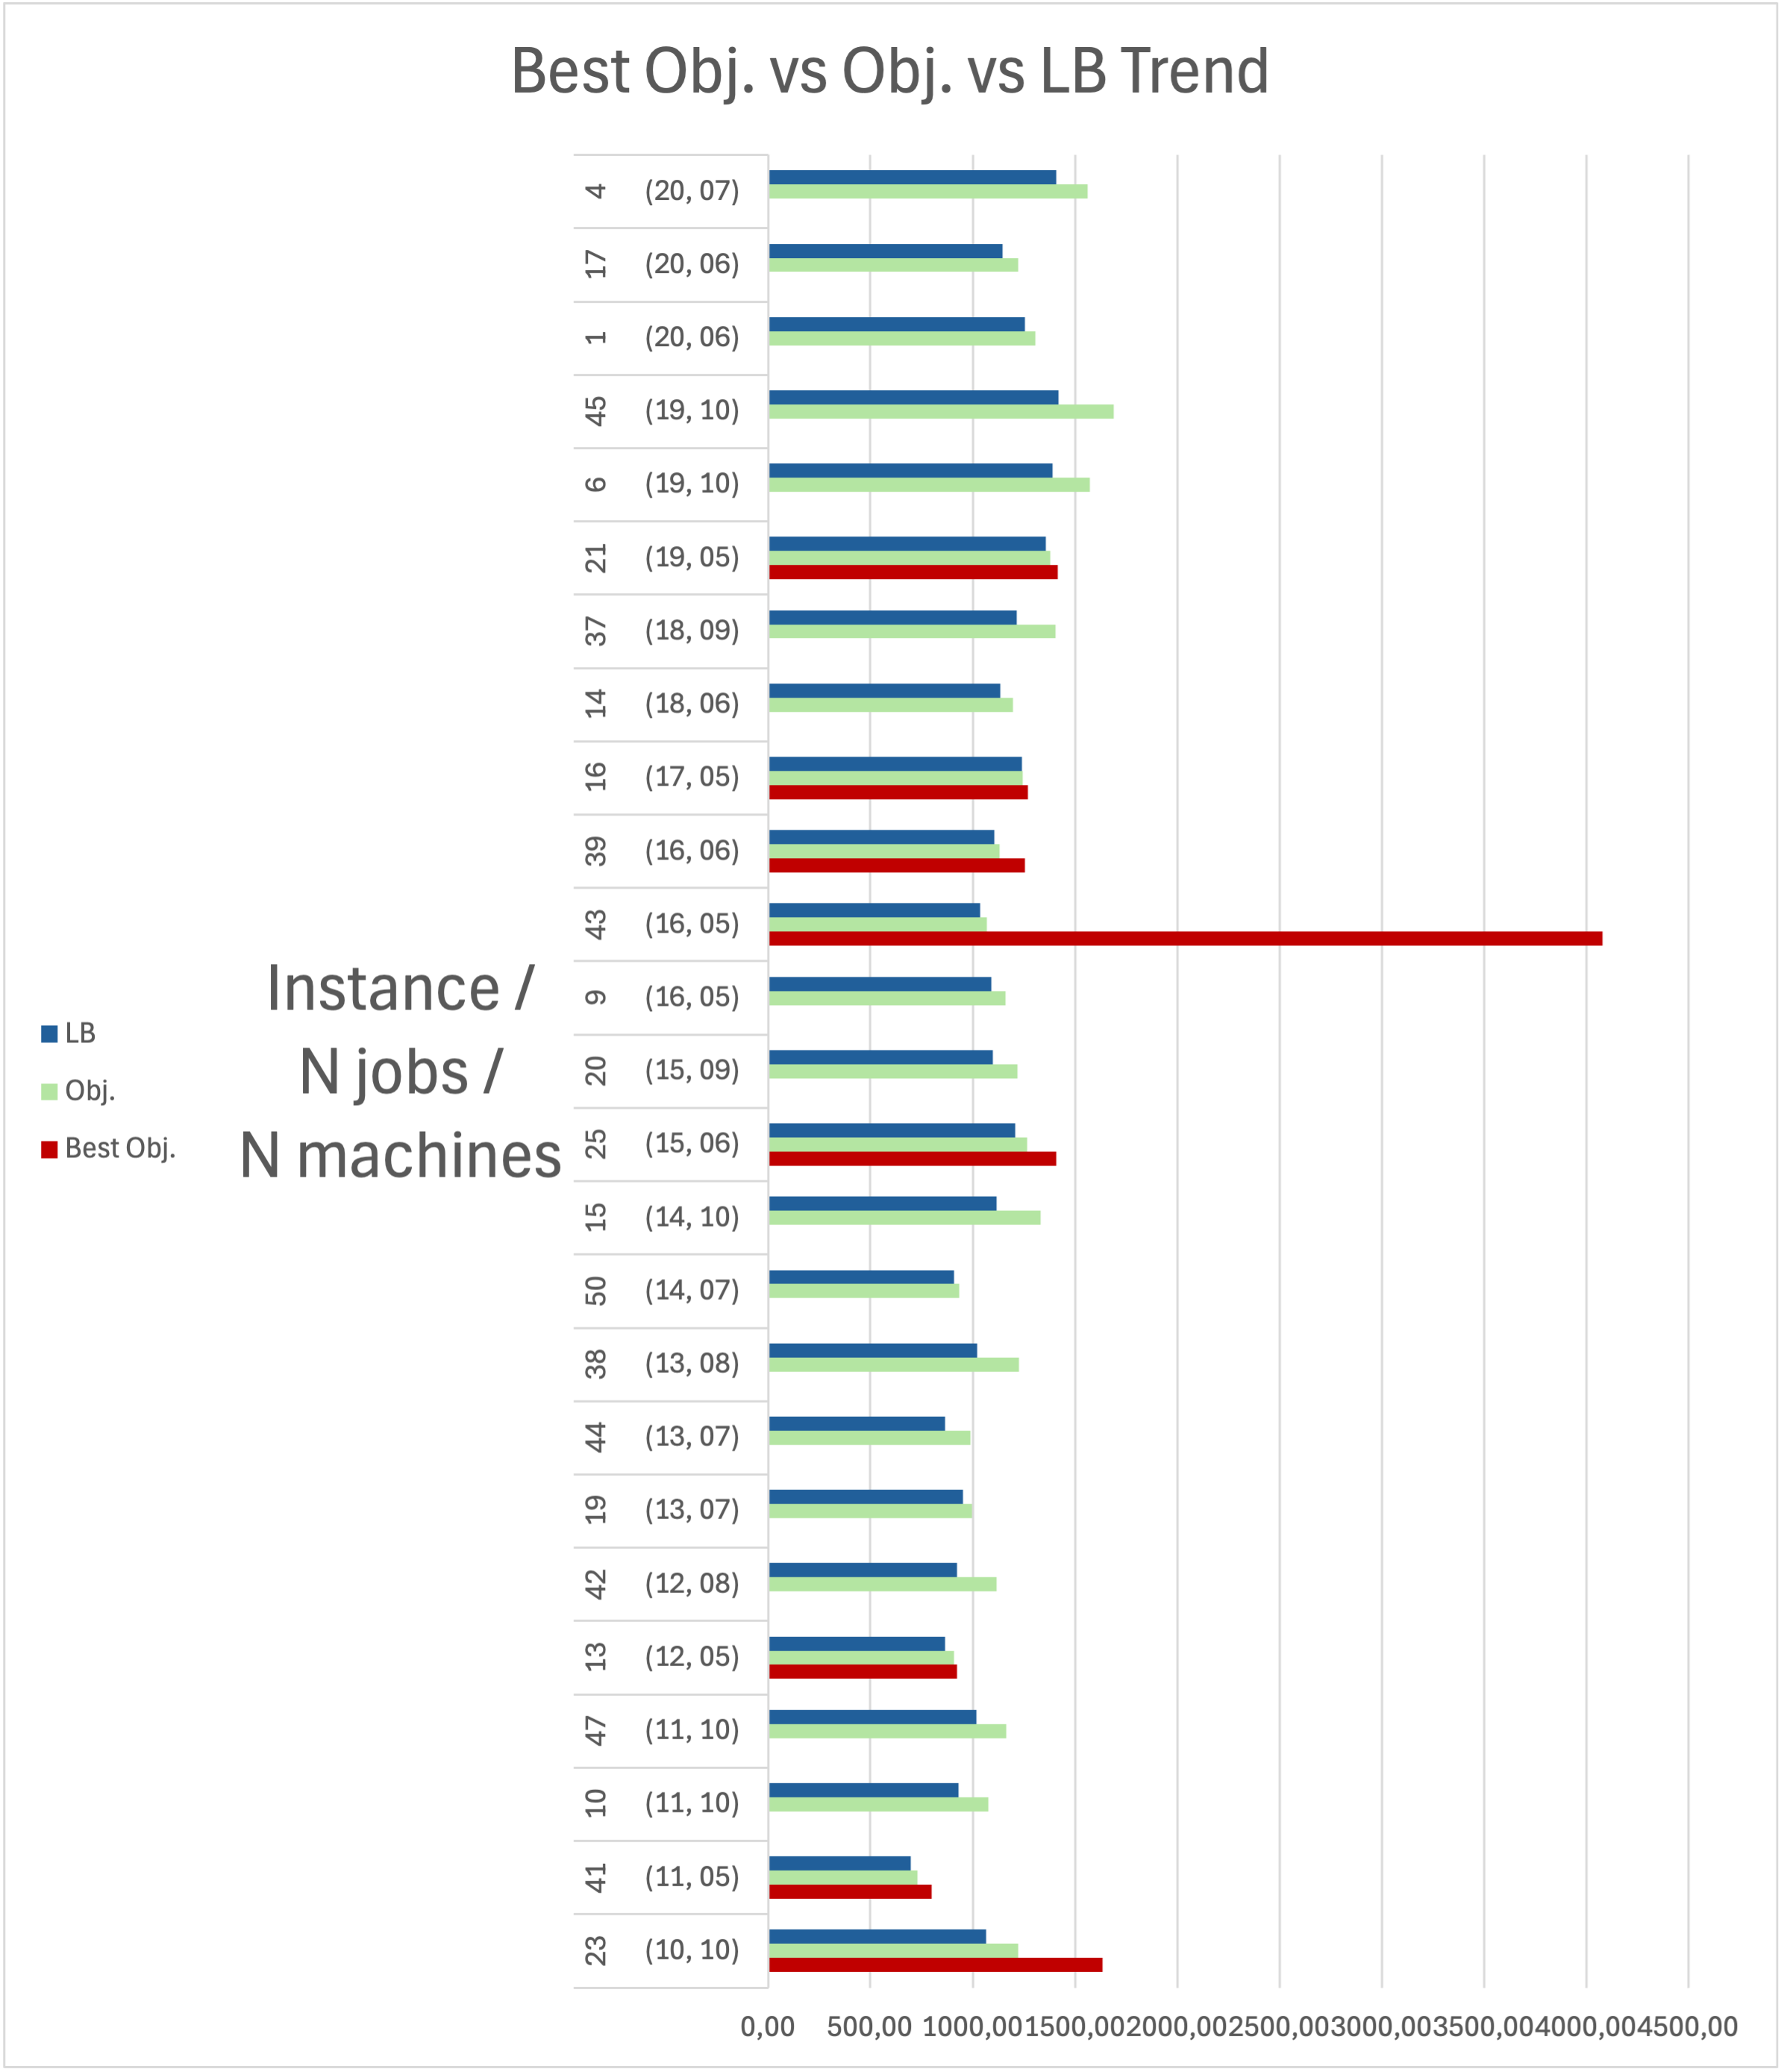
\includegraphics[width=0.95\textwidth]{images/obj_histogram_2.png}
    \caption{Representation of the objective values in an histogram}
    \label{fig:obj_histogram_2}
\end{figure}

\begin{figure}
    \centering
    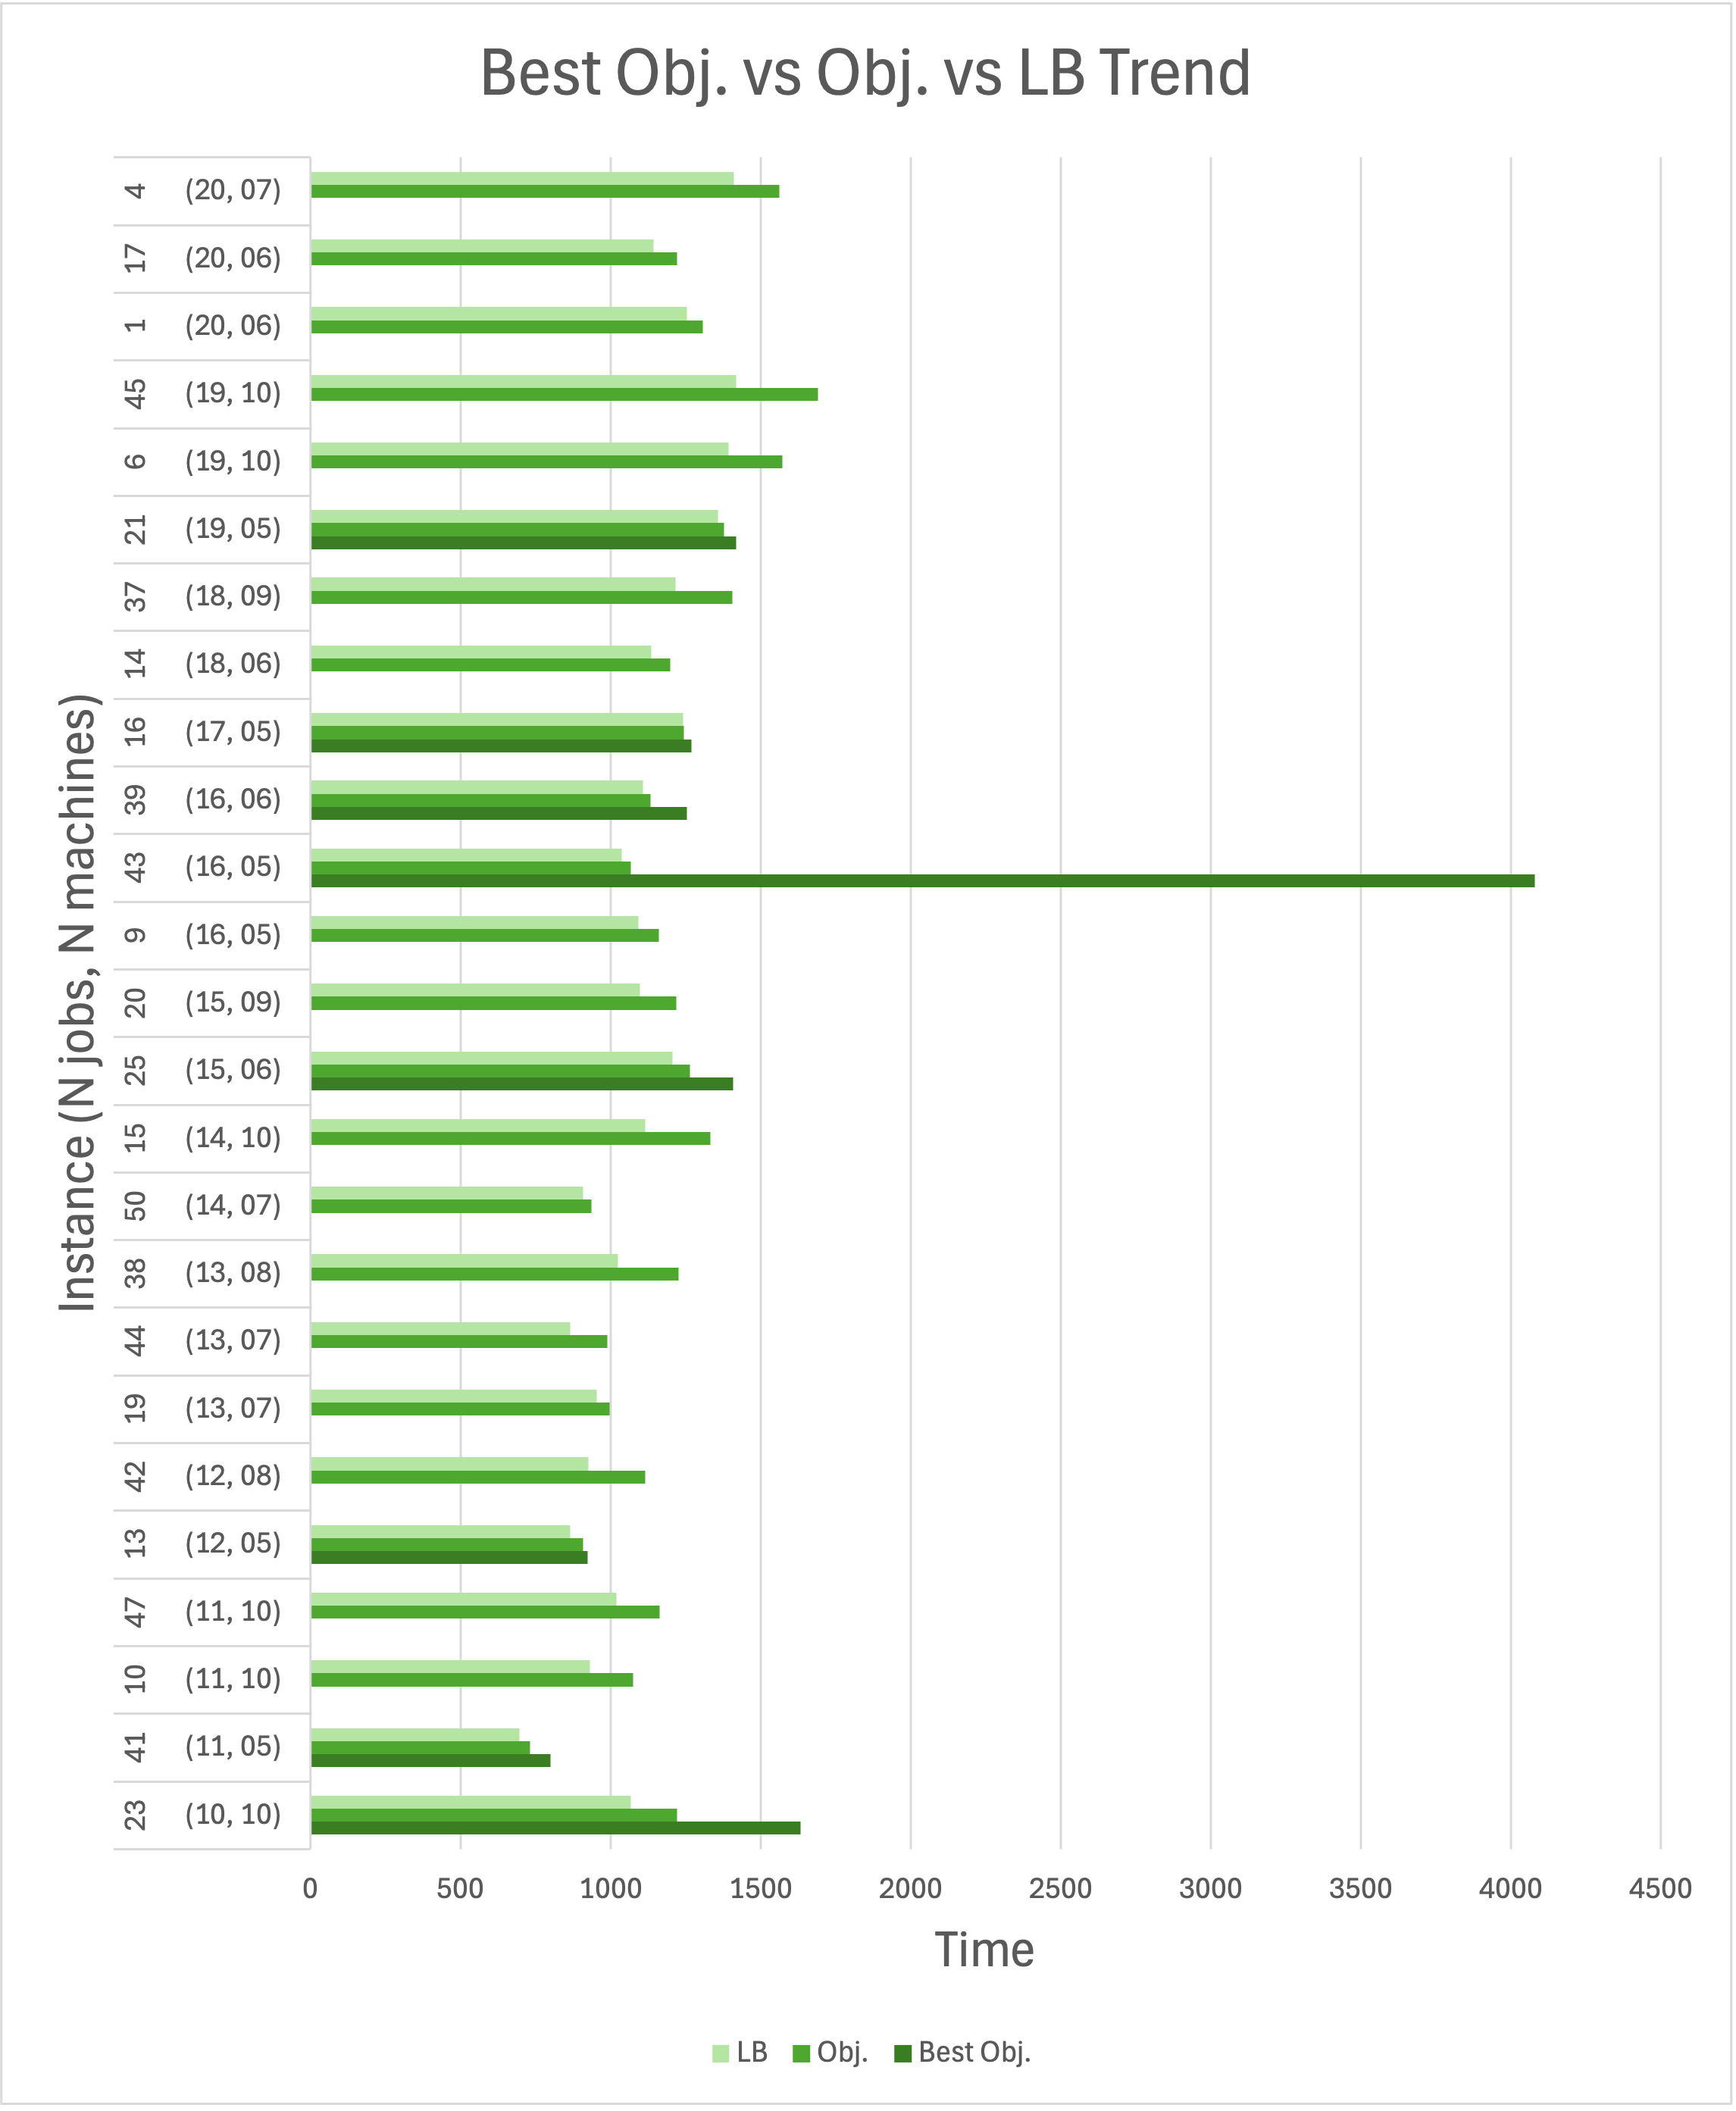
\includegraphics[width=0.95\textwidth]{images/obj_histogram_1.png}
    \caption{Representation of the objective values in an histogram}
    \label{fig:obj_histogram_1}
\end{figure}

The results show that the exact algorithm frequently reaches the maximum time, set on 300 seconds (exactly \textbf{74\%} of the times). That means that it gets lost analyzing all the branches of the search tree, sometimes not even finding a feasible solution. Indeed \textbf{42\%} of the times it doesn't find a solution and \textbf{34\%} of the times it finds a feasible solution. Instead the metaheuristic reaches the solution with a \textbf{100\%} success rate within few seconds.

Furthermore, when the MIP algorithm finds the best solution (within the 300 seconds, the \textbf{24\%} of the times) the objective value is always the same as the metaheuristic one implements.

The LB value moreover is always equal or less than the optimal solution and the metaheuristic solution. But the LB is just a minimal theoretical value that the function could reach if it was given more time. It is not the actual optimal solution. That's why the metaheuristic could have actually given the optimal solution without knowing it.

\subsection{Computational Time Analysis}

\textbf{Line graph \ref{fig:calculus_time}} shows an analysis on the computational time reached by the MIP solver and the metaheuristic.

\begin{figure}
    \centering
    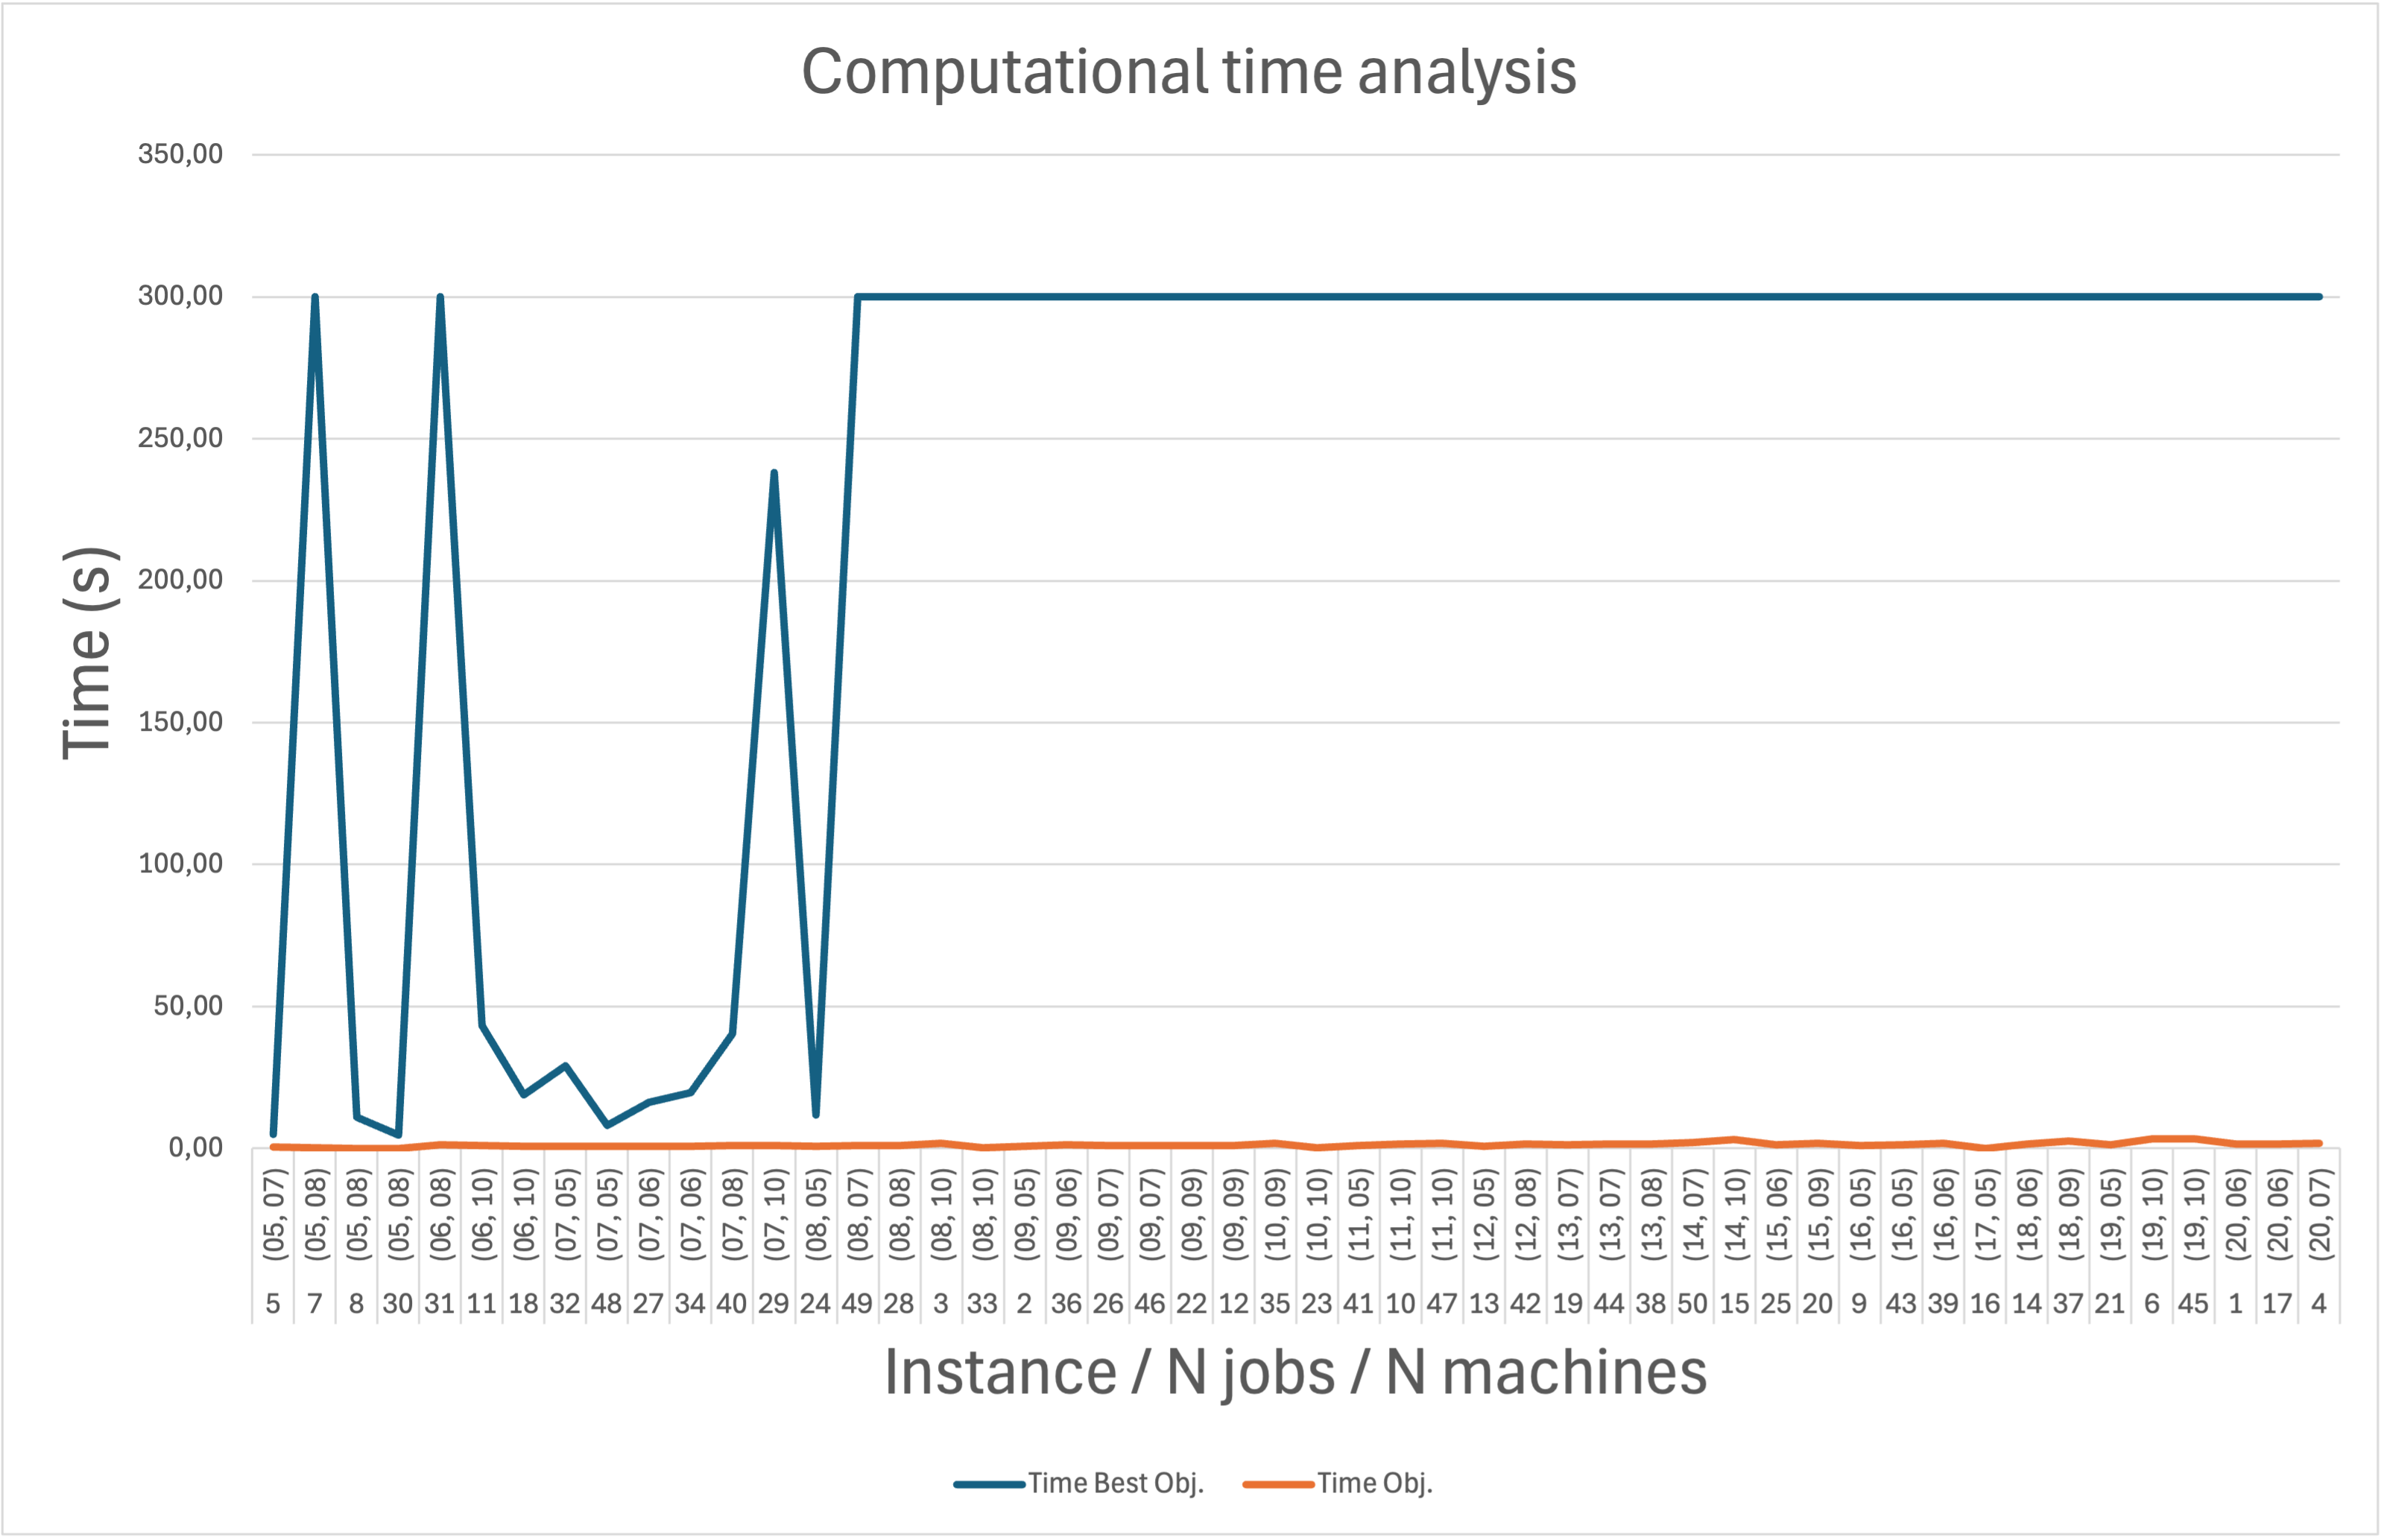
\includegraphics[width=0.95\textwidth]{images/calculus_time.png}
    \caption{Representation of the computational times in a line graph}
    \label{fig:calculus_time}
\end{figure}

It is clearly visible that, as the number of jobs ad of machines grows, the metaheuristic has a very small variation of the time spent while the MIP solver reaches the 300 seconds very rapidly.

\subsection{\% Gap Analysis}

\textbf{Line graph \ref{fig:perc_gap}} shows an analysis on the percentage gaps between the Obj. and the Best Obj. and between the LB and the Obj.

\begin{figure}
    \centering
    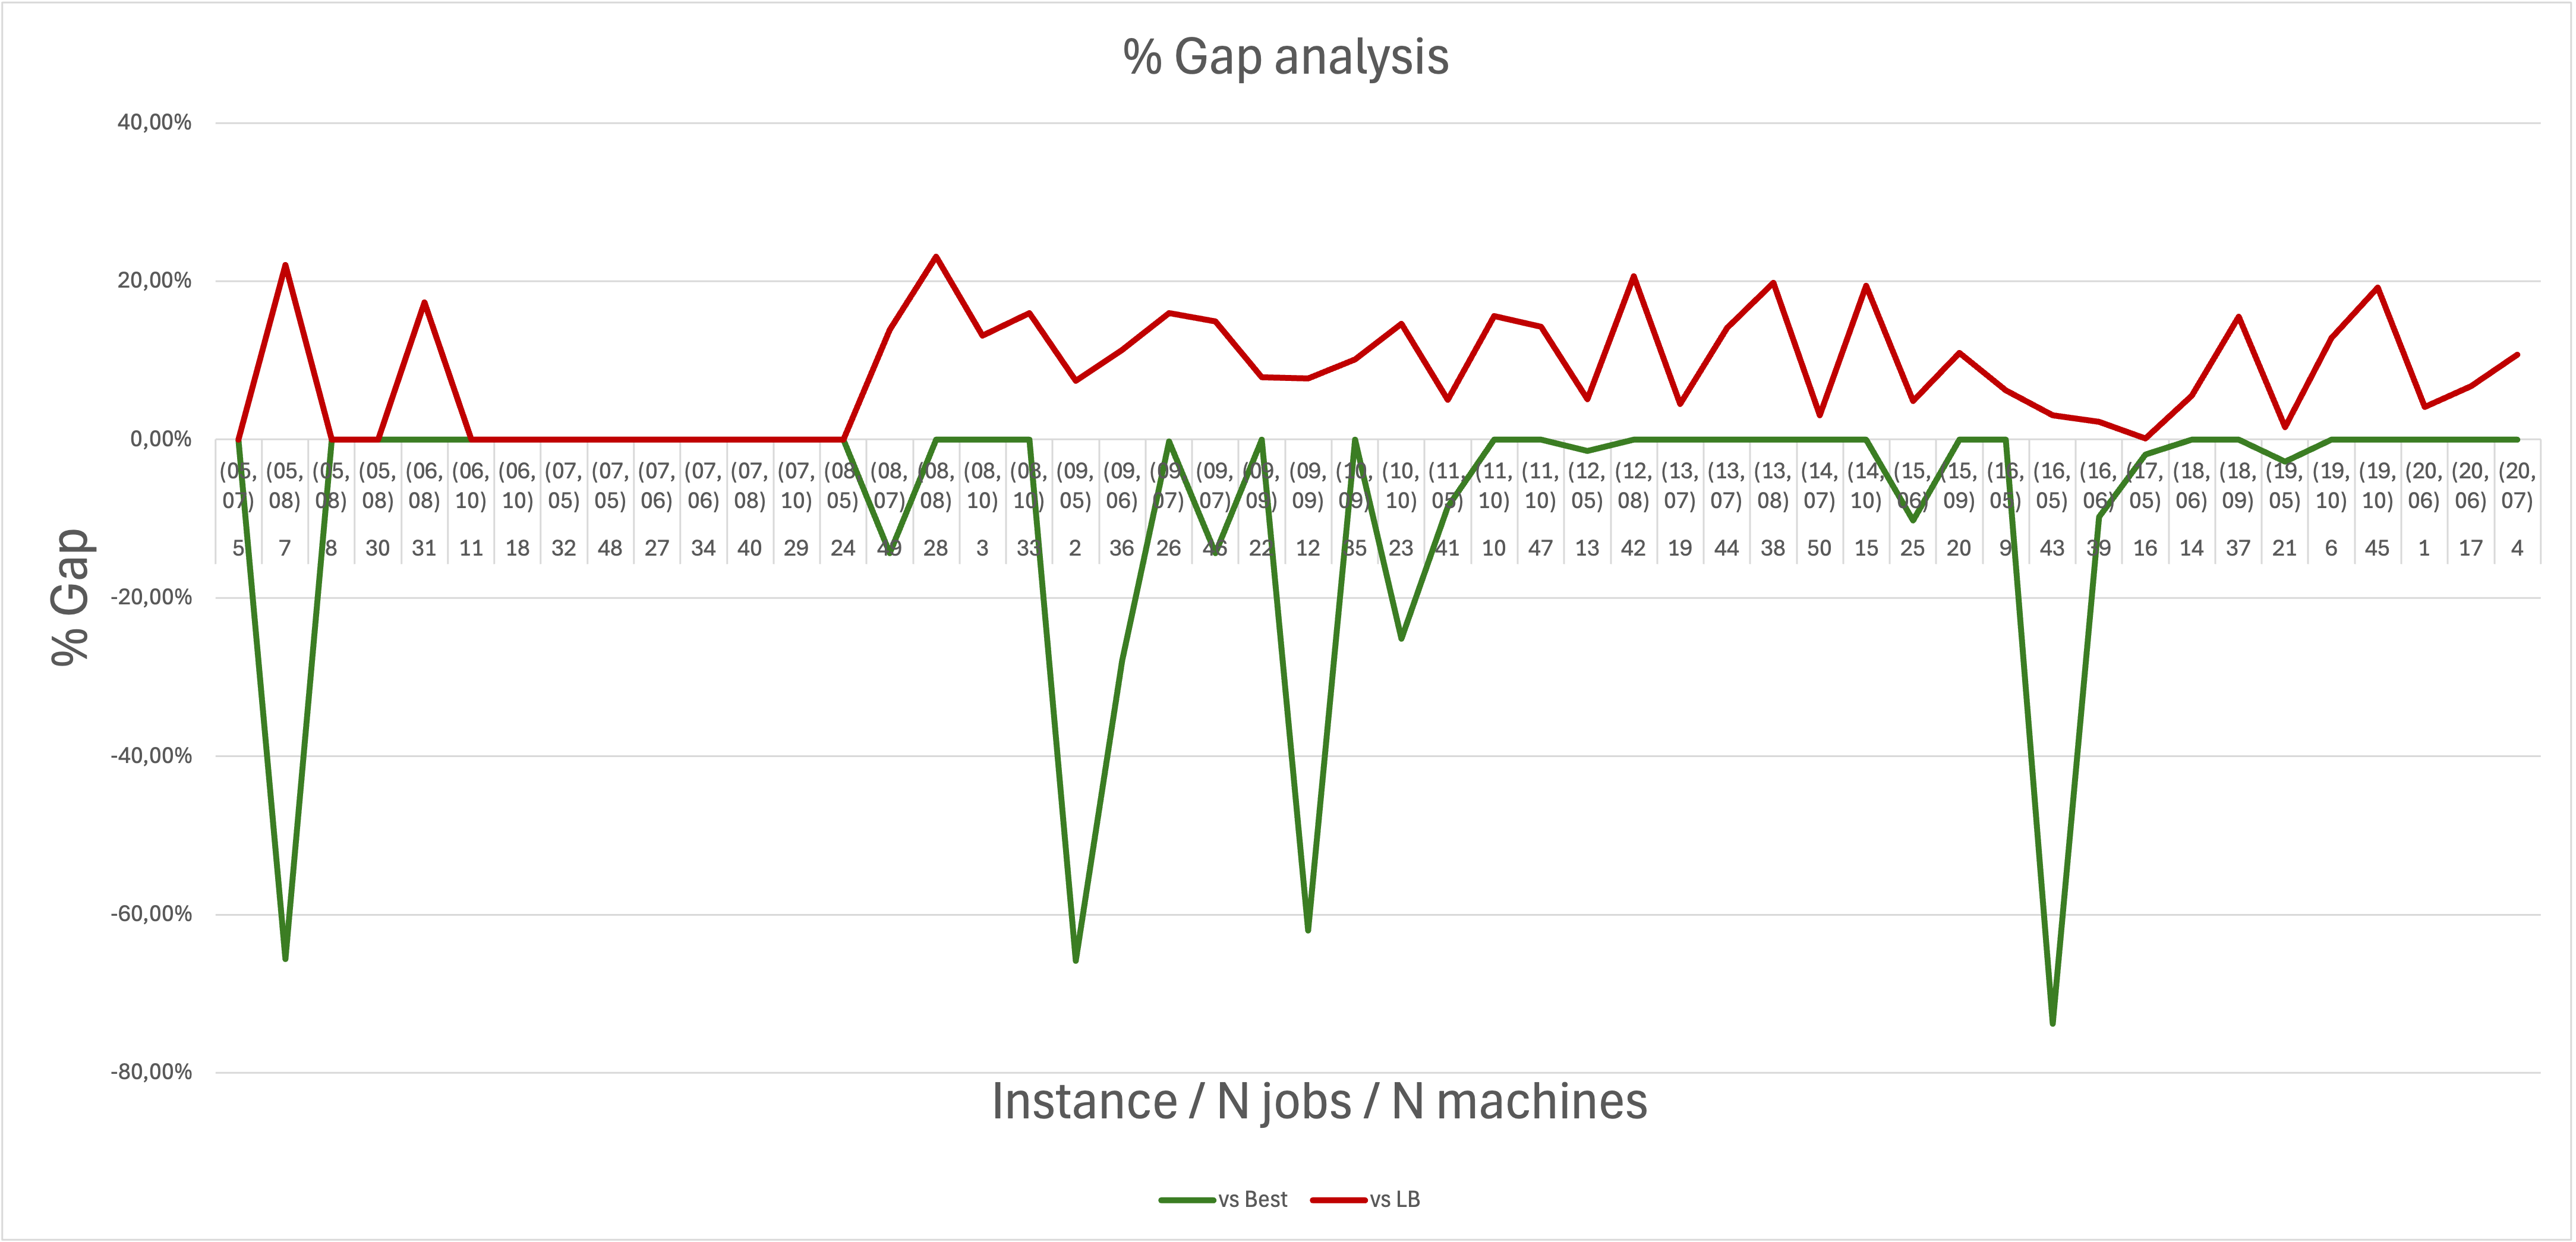
\includegraphics[width=0.95\textwidth]{images/perc_gap.png}
    \caption{Representation of the percentage gaps in a line graph}
    \label{fig:perc_gap}
\end{figure}

In the points where the lines coincide on the zero the MIP solver has reached the optimum in the 300 seconds timer. While where the "vs Best" reaches the zero value but the "vs LB" doesn't, represent the instances in which the MIP solver couldn't find a feasible solution.

The "vs LB" indicates that the percentage is always positive while the "vs Best" is always negative. That means that the LB value is always better or equals to the Obj. value of the metaheuristic while the Best Obj. value of the MIP solver is always equal or worse to the Obj. value of the metaheuristic.